\chapter{INTRODUCTION}

\section{Background}
Geographic positioning in the Himalayas is often unreliable due to GNSS signal blockage in deep valleys. However, the mountain skyline provides a stable geometric reference for navigation \cite{Pan2020}. A camera-based system can determine location by matching photo skylines against a database of horizons generated from Digital Elevation Models (DEMs) \cite{Steger2022, Pan2020}.

\section{Motivation}
In high-altitude regions like Khumbu, navigation failure can be life-threatening. Since portable devices are common, using their cameras for offline positioning provides a robust backup to satellite systems. This technology is essential for trekkers and search-and-rescue teams operating in areas with poor signal reception or GNSS denial.


\section{Problem Statement}
The objective is to estimate a camera's location and orientation using only the visible mountain skyline. The system must address several real-world challenges:
\begin{enumerate} 
\item \textbf{Extraction:} Haze, clouds, and low contrast frequently obscure the skyline boundary in real-world photographs \cite{Yang2025}. 
\item \textbf{Search Scale:} Matching a partial skyline against a massive 360-degree database is computationally expensive without prior orientation data \cite{Pan2020}. 
\item \textbf{Data Scarcity:} Annotated mountain photographs are scarce for the Himalayas, requiring the use of synthetic terrain views for training extraction models \cite{Brejcha2017}. 
\end{enumerate}

\section{Objectives}
The core objectives are: 
\begin{itemize}
\item To generate a 360-degree horizon database from high-resolution elevation models.
\item To implement a matching pipeline using Euclidean distance and Dynamic Time Warping (DTW) to resolve geographic coordinates from photos.
\end{itemize}


\section{Scope and Limitations}
The study focuses on a $36.4\text{ km} \times 31.2\text{ km}$ area in the Khumbu region of Nepal. 
\begin{itemize} 
\item \textbf{Northwest (NW):} $86.600^{\circ}\text{E}$, $28.050^{\circ}\text{N}$ 
\item \textbf{Northeast (NE):} $86.970^{\circ}\text{E}$, $28.050^{\circ}\text{N}$ 
\item \textbf{Southwest (SW):} $86.600^{\circ}\text{E}$, $27.770^{\circ}\text{N}$ 
\item \textbf{Southeast (SE):} $86.970^{\circ}\text{E}$, $27.770^{\circ}\text{N}$
\end{itemize}

\begin{figure}[h]
    \centering
    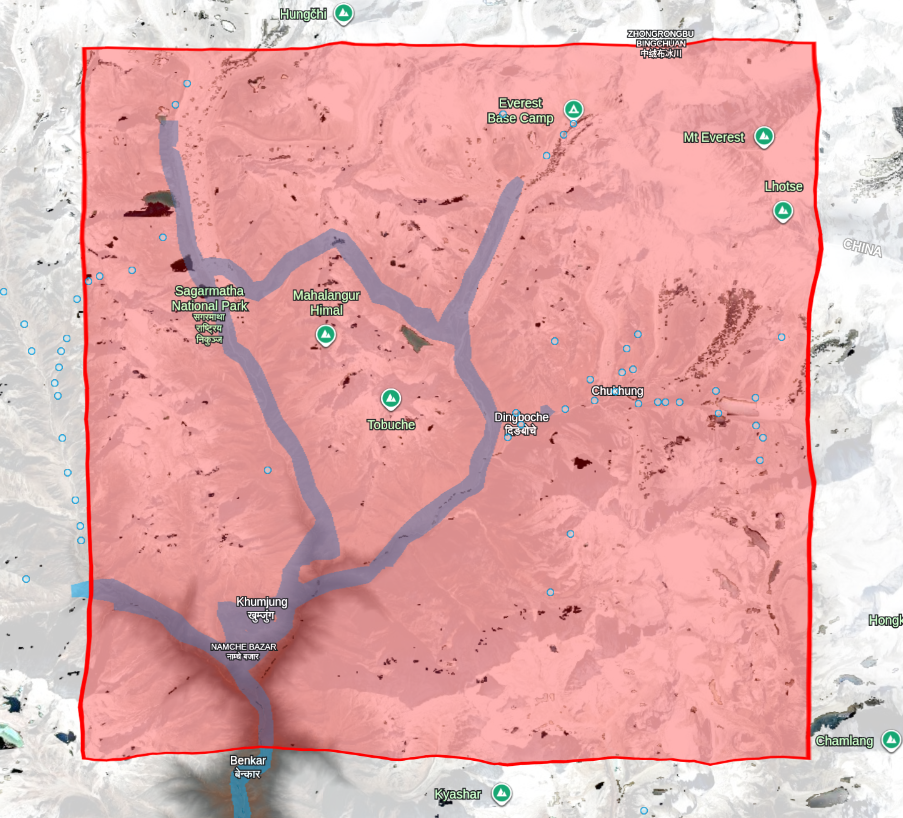
\includegraphics[width=0.8\textwidth]{src/images/roi.png}
    \caption{Region of Interest (ROI)}
    \label{fig:roi}
\end{figure}

The system is designed for offline use on standard portable hardware. Limitations include a focus on primary skylines and failures in cases where weather or obstacles completely block the view.


